\subsubsection{Struttura}
Lo strato di trasporto virtuale è visto dall'esterno come una black box che 
prende in ingresso messaggi dal livello applicativo, e restituisce i messaggi
di risposta dell'host interlocutore.\\
Nello specifico un messaggio viene frammentato in segmenti di una misura 
massima prefissata (MSS), i quali poi vengono inviati e gestiti tramite 
l'algoritmo di trasferimento affidabile, in questo modo vi è la garanzia che 
un segmento non venga ulteriormente suddiviso a livello di collegamento.\\
La dimensione massima del segmento è stata calcolata considerando un MTU 
relativo ad un collegamento Ethernet standard di 1500 byte, un header UDP/IP
di 28 byte ed un header contente i parametri necessari all'esecuzione 
dell'algoritmo: il numero di sequenza del segmento pari ad 1 byte e la 
quantità di byte significativi nel payload pari a 2 byte.
Il numeri di sequenza sono contenuti in variaili da 8 bit, pertanto vanno 
da $0$ a MAXSEQNUM - 1, con MAXSEQNUM = $2^8$.

%MSS = MTU - UDP/IP - SR
\begin{lstlisting}[title=transport.h]

#define MAXSEQNUM       (1 << 8)
#define MTU             1500
#define UDPIP_HEADER    28
#define SR_HEADER       (sizeof(uint8_t) + sizeof(uint16_t))

#define MSS             (MTU - UDPIP_HEADER - SR_HEADER)


struct segment {
	uint8_t  seqnum;
	uint16_t size;
	uint8_t  payload[MSS];
};
\end{lstlisting}

Il livello di trasporto virtuale è composto principalmente da due servizi 
indipendenti:
\begin{itemize}
\item \textbf{send\_service}: servizio che si occupa dell'invio dei segmenti e
della gestione di gran parte del protocollo lato mittente.
\item \textbf{recv\_service}: servizio che si occupa principalmente della
ricezione di ack e segmenti, pertanto interpreta il lato destinatario del 
protocollo e collabora con il lato mittente.
\end{itemize}
Entrambi vengono implementati tramite thread, per renderli indipendenti dal 
thread principale ``applicativo'' e affinché sia possibile che un host invii 
segmenti e riceva ACK contemporaneamente.\\
L'operazione di creazione di questi thread, sia lato mittente che destinatario
(con gli stessi parametri), equivale all'instaurazione della connessione,
e viene eseguita dalla funzione \emph{init\_transport}.

\begin{lstlisting}[title=transport.c]
/* shared structures */
struct circular_buffer recv_cb;
struct circular_buffer send_cb;
struct event e;
/* threads args to keep alive */
struct shared_tools recv_tools, send_tools;


void init_transport(int sockfd, struct proto_params *params)
{
    pthread_t t;

    /* initialize circular buffers */

    recv_cb.E = recv_cb.S = 0;
    send_cb.E = send_cb.S = 0;

    /* initialize shared tools */

    recv_tools.sockfd = sockfd;
    recv_tools.e = &e;
    recv_tools.cb = &recv_cb;
    recv_tools.params = params;

    send_tools = recv_tools;
    send_tools.cb = &send_cb;

    /* initialize mutexes */

    if (pthread_mutex_init(&e.mtx, NULL) != 0)
        handle_error("pthread_mutex_init()");
    if (pthread_mutex_init(&recv_cb.mtx, NULL) != 0)
        handle_error("pthread_mutex_init()");
    if (pthread_mutex_init(&send_cb.mtx, NULL) != 0)
        handle_error("pthread_mutex_init()");

    /* initialize conditions */

    if (pthread_cond_init(&recv_cb.cnd_not_empty, NULL) != 0)
        handle_error("pthread_cond_init()");
    if (pthread_cond_init(&send_cb.cnd_not_empty, NULL) != 0)
        handle_error("pthread_cond_init()");

    if (pthread_cond_init(&recv_cb.cnd_not_full, NULL) != 0)
        handle_error("pthread_cond_init()");
    if (pthread_cond_init(&send_cb.cnd_not_full, NULL) != 0)
        handle_error("pthread_cond_init()");

    if (pthread_cond_init(&e.cnd_event, NULL) != 0)
        handle_error("pthread_cond_init()");
    if (pthread_cond_init(&e.cnd_no_event, NULL) != 0)
        handle_error("pthread_cond_init()");

    /* create threads */

    if (pthread_create(&t, NULL, recv_service, &recv_tools) != 0)
        handle_error("creating recv_service");

    if (pthread_create(&t, NULL, send_service, &send_tools) != 0)
        handle_error("creating send_service");
}
\end{lstlisting}

Il servizio di invio è stato implementato come un thread che rimane in attesa
fintanto che non avviene uno dei seguenti eventi:
\begin{itemize}
\item[-]Ricezione dati dal livello applicativo;
\item[-]Ricezione di un aknowledgment dalla rete;
\item[-]Scadenza di un timeout relativo ad un segmento inviato.
\end{itemize}

Il sistema di attesa è stato implementato tramite un meccanismo di segnalazione
di eventi basato su variabili di condizione.\\
Il thread infatti attende fintanto che non viene segnalata una condizione di
evento, dopodiché esso si sveglia ed in base al tipo di evento 
esegue il compito associato.\\
La struttura \emph{event} è composta dalle due variabili condizione 
\emph{cond\_event} e \emph{cond\_no\_event}, che indicano rispettivamento
il verificarsi di un evento ed il caso opposto, ovvero che non vi è un evento
da gestire, l'intero \emph{type} invece specifica il tipo di evento che si è
verificato e l'intero a 8 bit \emph{acknum} contiene il numero di sequenza del
segmento per il quale si è ricevuto un ack.
%
\begin{lstlisting}[title=event.h]
#define NO_EVENT	0
#define PKT_EVENT	1
#define ACK_EVENT	2

struct event {
	pthread_mutex_t mtx;
	pthread_cond_t cnd_event;
	pthread_cond_t cnd_no_event;
	unsigned int type;
	uint8_t acknum;
};

int cond_event_signal(struct event *e, unsigned int event_type);
int cond_ack_event_signal(struct event *e, uint8_t acknum);
\end{lstlisting}
%
La funzione \emph{cond\_event\_signal} permette di inviare un segnale che indica il
verificarsi della condizione \emph{cond\_event} relativa ad uno specifico tipo di 
evento.\\
La funzione \emph{cond\_ack\_event} è relativa soltanto all'avento di ricezione
di un ack, e permette, oltre che di segnalare l'evento, anche di specificare
il numero di sequenza del segmento per il quale si è ricevuto l'ack.
In questo modo vengono segnalati gli eventi di consegna di dati dall'applicazione
e di arrivo di un ack.\\
La scadenza di un timeout invece avviene semplicemente 
impostando un tempo limite di attesa per la funzione \emph{pthread\_cond\_timedwait},
al termine del quale il thread si risveglia e verrà restituito il valore ETIMEDOUT 
che indica tale evento.
%
\begin{lstlisting}[title=transport.c]
void *send_service(void *p)
{
		.......

    if (pthread_mutex_lock(&e->mtx) != 0)
        handle_error("pthread_mutex_lock");

    for (;;) {

        e->type = NO_EVENT;
        if (pthread_cond_broadcast(&e->cnd_no_event) != 0)
            handle_error("pthread_cond_broadcast()");

        condret = 0;
        while (e->type == NO_EVENT && condret != ETIMEDOUT) {
            // no events and timeout not expired

		.......

            condret = pthread_cond_timedwait(&e->cnd_event,
                      &e->mtx, &wait_time);
            if (condret != 0 && condret != ETIMEDOUT)
                handle_error("pthread_cond_timedwait");
        }

        /* TIMEOUT EVENT */
        if (condret == ETIMEDOUT) {
            // timeout work .......
            continue;
        }

        switch (e->type) {

        case PKT_EVENT:
            // pkt work .......
            break;

        case ACK_EVENT:
            // ack work .......
            break;
        }
    }

    if (pthread_mutex_unlock(&e->mtx) != 0)
        handle_error("pthread_mutex_unlock");

		.......
}
\end{lstlisting}
%
L'accesso esclusivo alla variabile \emph{event} è garantito dalla presenza
del mutex come attributo della stessa.\\
Il thread di invio acquisisce il mutex appena viene instaurata la connessione
e lo rilascia soltanto tramite la \emph{pthread\_cond\_timedwait}, ovvero
quando si mette in attesa di un evento, pertanto non è possibile che la 
variabile venga acceduta durante la gestione di uno degli eventi.\\
Per quanto riguarda la concorrenza tra il thread principale e il thread di
ricezione, il primo che accede alla variabile tramite l'acquisizione del
mutex segnala il proprio evento, poi se il secondo accede e trova che il tipo
di evento è diverso da NO\_EVENT aspetta fintanto che il thread di invio 
non se ne occupa e segnala di nuovo l'assenza di eventi tramite la funzione
\emph{pthread\_cond\_broadcast}, a questo punto è possibile segnalare l'evento
successivo. In altre parole, prima di seganalare un evento, un thread attende 
che un eventuale evento segnalato precedentemente venga gestito.
%
\begin{lstlisting}[title=event.c]
int cond_event_signal(struct event *e, unsigned int event_type)
{
    int retval = 0;

    if (pthread_mutex_lock(&e->mtx) != 0)
        retval = -1;

    else {

        // wait until no event is signaled
        while (e->type != NO_EVENT)
            if (pthread_cond_wait(&e->cnd_no_event, &e->mtx) != 0)
                retval = -1;

        e->type = event_type;

        if (pthread_cond_signal(&e->cnd_event) != 0)
            retval = -1;

        if (pthread_mutex_unlock(&e->mtx) != 0)
            retval = -1;
    }

    return retval;
}
\end{lstlisting}


Il servizio di ricezione invece risponde ai seguenti eventi:
\begin{itemize}
\item[-]Ricezione di dati dalla rete (segmenti o ack);
\item[-]Scadenza di un timeout relativo alla connessione.
\end{itemize}
In caso di ricezione di dati dalla rete, segmenti e ack vengono distinti in 
base alla loro dimensione, invece il timeout è implementato impostandolo
sulla socket in lettura.
%
Il servizio di ricezione invece risponde ai seguenti eventi:
\begin{itemize}
\item[-]Ricezione di dati dalla rete (segmenti o ack);
\item[-]Scadenza di un timeout relativo alla connessione.
\end{itemize}
%
In caso di ricezione di dati dalla rete, segmenti e ack vengono distinti in 
base alla loro dimensione, invece il timeout è implementato impostandolo
sulla socket in lettura.
%
\begin{lstlisting}[title=transport.c]
void *recv_service(void *p)
{
	.....

    for (;;) {

        r = read(sockfd, buffer, max_recvsize);

        if (r == -1) {
            if (errno == EINTR)
                // signal interruption
                continue;
            if (errno == EAGAIN || errno == EWOULDBLOCK) {
                // timeout expired: close connection
                puts("Connection expired\n");
                exit(EXIT_SUCCESS);
            }
            handle_error("recv_service - read()");
        }

        /* segment received */
        if (r == sizeof(struct segment)) {

            // segment work .....
            
            continue;
        }

        /* ACK received */
        if (r == sizeof(acknum)) {

            // ack work .....

            continue;
        }

        fputs("recv_service: undefined data received\n", stderr);
    }

	.....
}
\end{lstlisting}


Le funzioni \emph{rdt\_send} e \emph{rdt\_recv} fungono da regolatori del flusso
di dati dal livello applicativo puro a quello di trasporto virtuale e 
viceversa.\\
Queste funzioni comunicano con i thread di invio e ricezione tramite 
dei buffer condivisi secondo uno schema del tipo produttore-consumatore, in 
modo tale che i dati effettuino il passaggio di livello solo quando c'è spazio
disponibile sui buffer.

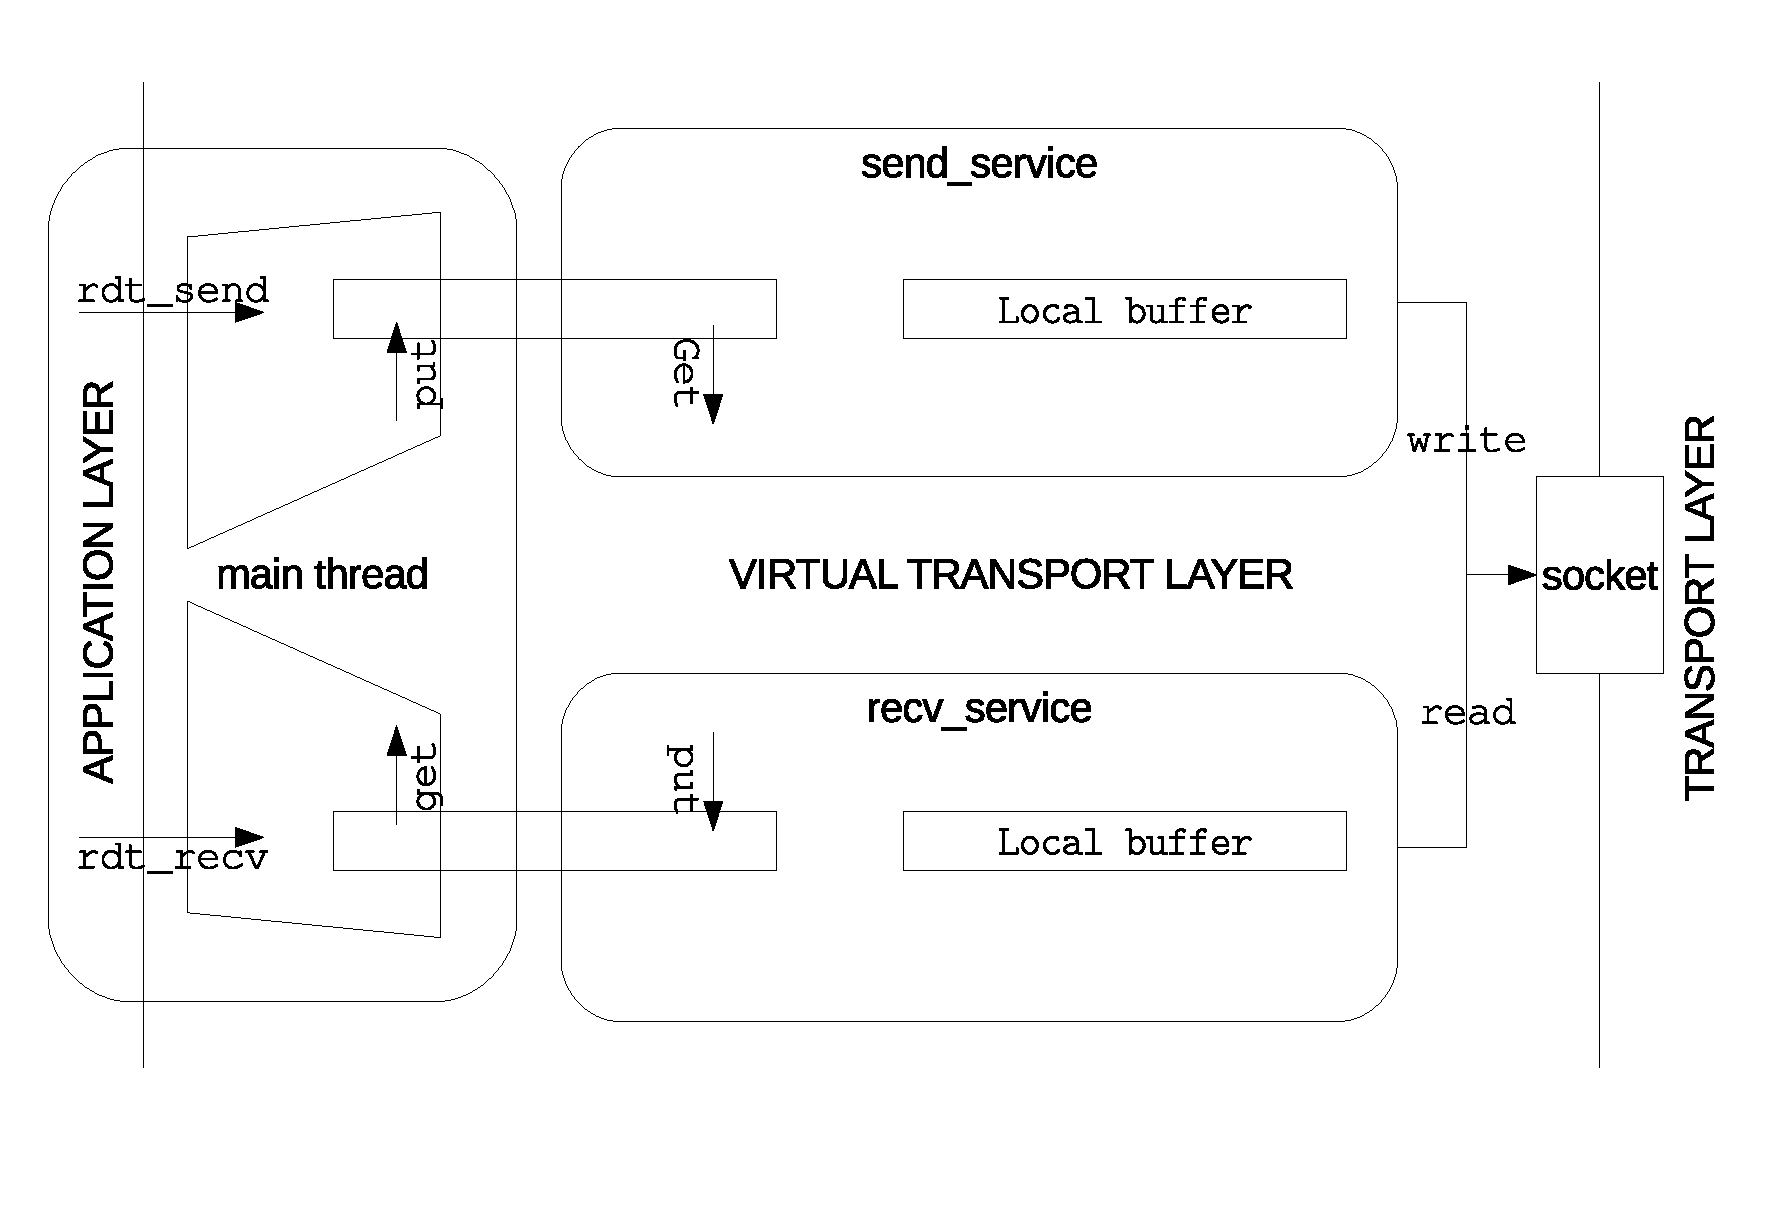
\includegraphics[scale=0.35]{images/structure_1}

Prima di passare a come viene implementato il \emph{selective repeat}, è 
necessario introdurre le strutture principali che ne supportano il 
funzionamento.\\
Come già detto, le unità di base con cui l'algoritmo ha a che fare sono
i segmenti che contengono i dati applicativi. Poiché tali segmenti sono
soggetti a ritrasmissioni, è necessario che vengano ``immagazzinati'' da 
qualche parte, inoltre, per quanto riguarda il lato destinatario, vanno
consegnati al livello applicativo in ordine, per queste ragioni, sia il 
servizio di invio che il servizio di ricezione sono dotati di buffer locali.\\
Tali buffer sono implementati tramite array di dimensione fissa e hanno una
capacità pari a MAXSEQNUM slot, in modo tale da far
corrispondere gli indici ai numeri di sequenza dei segmenti e 
garantirne un accesso immediato ($\mathcal{O}(1)$). Inoltre i buffer vengono
trattati come circolari, così da emulare naturalmente il riciclo dei numeri 
di sequenza.\\
Mentre il buffer del \emph{recv\_service} è implementato tramite un'array di 
strutture \emph{segment}, quello del \emph{send\_service} è un'array di 
strutture \emph{packet}, ovvero contenitori di segmenti e informazioni ad essi
relative necessarie al funzionamento del timeout, come istante di invio, quello
di scadenza ed un booleano che indica se il pacchetto è stato ritrasmesso.

\begin{lstlisting}[title=transport.h]
struct packet {
	struct segment sgt;
	struct timespec sendtime;
	struct timespec exptime;
	bool rtx;
};
\end{lstlisting}

Un'altra struttura fondamentale per l'algoritmo è la \emph{window}, che 
rappresenta le finestre di spedizione o ricezione delle due parti 
coinvolte.
\begin{lstlisting}[title=window.h]
struct window {
	unsigned int base;
	unsigned int width;
	struct bit_array ack_bar;	// 128 bit array
};
\end{lstlisting}
Tale struttura è composta da un'indice \emph{base} che rappresenta la base
della finestra, un intero \emph{width} che indica l'ampiezza massima della
finestra ed infine una struttura \emph{bit\_array} che non è altro che una
bitmask che tiene conto di quali segmenti sono arrivati a destinazione a 
partire dalla base della finestra.

[Disegno esempio bitmask] 

Infine, vi è la struttura necessaria alla gestione del timeout dei segmenti
inviati: una coda prioritaria i cui nodi sono puntatori
ai pacchetti presenti nel buffer locale di invio.\\
Ogni nodo è ordinato in base alla scadenza del timeout e una scansione 
periodica determina quali segmenti vanno ritrasmessi, appena si trova un 
segmento non scaduto non è necessario controllare i successivi
nella coda.
Questo meccanismo permette di gestire più timeot logici avendo un solo 
contatore hardware a disposizione.\\
In termini di prestazioni, avendo già N nodi nella coda, 
l'inserimento di un nuovo nodo richiede il confronto con tutti i
nodi che scadono prima, questo si effettua al più con un numero di passi
pari al numero di nodi presenti ($\mathcal{O}(N)$)
nel caso di timeout adattativo, invece se il timeout è costante non vi è bisogno
di alcun confronto poiché l'ultimo nodo inviato sarà l'ultimo a scadere e 
verrà semplicemente accodato (tempo $\mathcal{O}(1)$).
Per quanto riguarda l'estrazione del primo nodo da ritrasmettere, grazie 
all'inserimento prioritario, non è richiesta nessuna scansione, poiché il nodo 
in testa sarà il primo a scadere.\\
La coda è stata implementata in maniera tale da occupare meno memoria possibile,
infatti i nodi sono composti dagli indirizzi delle strutture \emph{packet}
presenti nel buffer locale, la coda tiene conto solo del loro ordinamento.

[disegno time\_queue]

